% !TEX root =  master.tex
\chapter{Optimierung und Potenziale}
\section{Optimierung der Poolgröße}
Im vorherigen Kapitel wurde aufgezeigt, dass die Effizienz einer Poolingmethode von zwei Parametern abhängt.
In Kombination ergeben diese beiden Werte die Wahrscheinlichkeit, mit welcher infizierte Personen innerhalb der Testgruppe sind.
\begin{itemize}
	\item \textbf{Prävalenz} Hieraus ergibt sich die Wahrscheinlichkeit, mit der Personen infiziert sind.
	Bei einem realen Testverfahren ist die Prävalenz ein externer Faktor.
	Sie ist Abhängig von der aktuellen Inzidenz und dem Umfeld der Testung.
	\item \textbf{Größe der Testgruppe} Diese kann vom Labor frei gewählt werden.
\end{itemize}

Dieser Zusammenhang ergibt die Funktion für den Erwartungswert:\newline
$\frac{Personenzahl}{(1 - (1-Prävalenz)^{Personenzahl} \cdot (Personenzahl + 1)) + ((1-Prävalenz)^{Personenzahl}) \cdot 1)}$

Für jede gegebene Prävalenz, lassen sich durch Auswahl der Personenanzahl unterschiedliche Verläufe der Effizienzkurve erreichen.
Die Anzahl der Personen pro Pool sollte deshalb anhand der Prävalenz gewählt werden, um den Erwartungswert zu maximieren.

Der Erwartungswert(Personenzahl, Prävalenz) lässt sich auch als Graph darstellen.
\begin{wrapfigure}{r}{0.48\textwidth}
	%\centering
	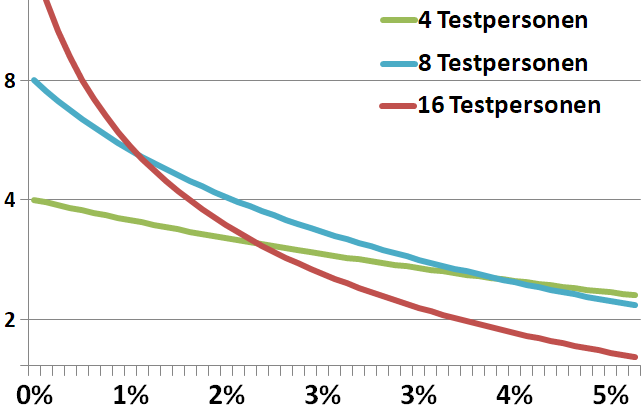
\includegraphics[width=.48\textwidth]{img/PraevalenzZuTestgruppe}
	\caption{\mbox{Effizienz unterschiedlicher} \mbox{Poolgrößen} nach Prävalenz\footnotemark}
\end{wrapfigure}
\footnotetext{Eigene Darstellung}
Wenn man eine der Variablen als Rahmenbedingung festsetzt, lässt sich der andere Wert gemeinsam mit der Effizienz als Diagramm zeichnen.
in Abbildung X.X wird die Personenanzahl auf 4, 8 und 16 festgesetzt und der Erwartungswert in Abhängigkeit der Prävalenz dargestellt.
Zu erkennen ist, dass höhere Personenzahlen bei niedrigen Prävalenzen die Effizienz enorm steigern können.
Wenn die Prävalenz allerdings steigt, werden die großen Pools schnell anfällig für Nachtestungen und verlieren so überproportional an Effizienz.

\cleardoublepage

Alternativ zur Darstellung nach Poolgröße kann auch die Prävalenz als gegeben festgesetzt werden.
In Abbildung X.X wird hierfür jedes Prävalenzniveau als eigener Graph dargestellt.
Das Optimum für die aktuelle Prävalenz liegt hierbei immer am Hochpunkt.
Die Poolgröße und hieraus resultierende Effizienz kann direkt auf den Achsen abgelesen werden.
\begin{figure}[h]
	\centering
	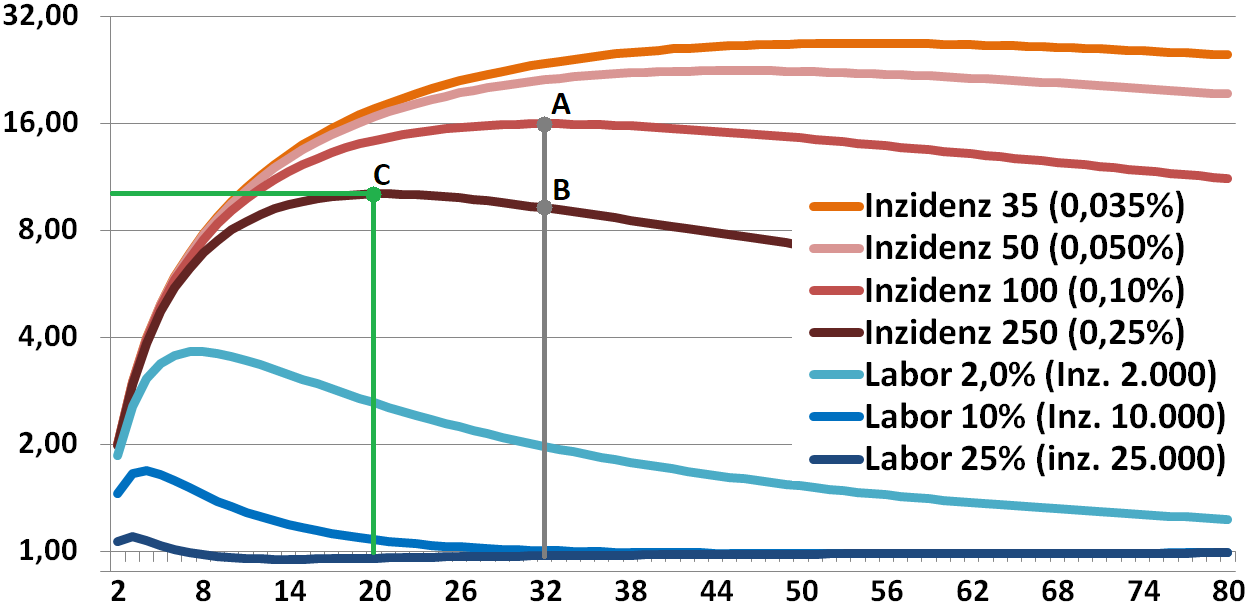
\includegraphics[width=1\textwidth]{img/EffizienzTestgruppePfeile}
	\caption{Effizienz eines Pools mit drei Personen nach Prävalenz\footnotemark}
\end{figure}
\footnotetext{Eigene Darstellung}

\begin{wraptable}{r}{7.7cm}
	\begin{tabular}{|r|r|c|r|}
		\hline
		Inzidenz&Prävalenz&Personen&Effizienz\\
		\hline
		35 & 0,00035 & 54 & 26,9x\\
		\hline
		50 & 0,00050 & 45 & 22,5x \\
		\hline
		100 & 0,00100 & 32 & 15,9x \\
		\hline
		250 & 0,00250 & 21 & 10,1x \\
		\hline
		2.000 & 0,02 & 8 & 3,6x\\
		\hline
		10.000 & 0,10  & 4 & 1,7x\\
		\hline
		25.000 & 0,25 & 3 & 1,1x\\
		\hline
	\end{tabular}
	\caption{Effizienzsteigerungspotenzial\footnotemark}
\end{wraptable} 
\footnotetext{Eigene Darstellung, Eine vollständige Gegenüberstellung in tabellarischer Form ist im Anhang dargestellt.}
Die bisherige Inzidenz lag bei 100.
Das Pooling an Punkt A war mit 32 Personen effizient und erreichte einen Faktor von 15,93.
Wenn die Inzidenz sich auf 250 erhöht, sinkt die Effizienz bei unveränderten Poolgröße auf Punkt B. Die Effizienz ist nur noch 9,24.
Für das neue Inzidenzniveau bei 250 kann das Pooling optimiert werden, indem die Poolgröße auf 20 gesenkt wird.
Dies bewirkt eine Linksverschiebung entlang der 250-Linie zu Punkt C.
Hier kann eine Effizienz von 10,12x erwartet werden.

\cleardoublepage

\section{Ausblick: Komplexe Poolingverfahren}
Dieser Abschnitt widmet sich einem Ausblick auf komplexere Poolingverfahren, welche im Umfang dieser Arbeit nicht näher beleuchtet werden können.
Durch die zunehmende Komplexität ergeben sich Potenziale für weitere Effizienzsteigerungen.
Diese sind allerdings auch mit neuen Risiken verbunden.

\textbf{Mehrdimensionale Pools}\ haben das Ziel, durch Überlappung der Pools den Bedarf einer Nachtestung bei einzelnen Positivfällen zu minimieren.
Die Testpersonen werden in einer AxB-Matrix angeordnet.
Die Proben werden dann für jede Spalte und jede Reihe gepoolt.
Allgemein formuliert lässt sich sagen:
Testbedarf pro Person =
$\frac{A+B}{A\cdot B}$

\begin{wrapfigure}{r}{0.48\textwidth}
	%\centering
	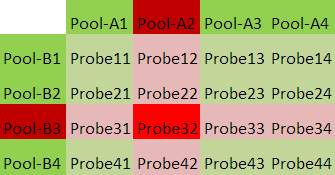
\includegraphics[width=.48\textwidth]{img/2d_Pool_1Positiv}
	\caption{Zweidimensionaler Pool mit einer positiven Probe\footnotemark}
\end{wrapfigure}
\footnotetext{Eigene Darstellung}
Für eine Testgruppe von 25 Personen, welche in einer 5x5 Matrix angeordnet sind, werden somit 5+5 Tests benötigt.
Die Effizienz läge bei 2,5x wenn alle Personen negativ getestet werden.
Vergleichen mit dem eindimensionalen Poolingverfahren klingt das zunächst nicht nach sehr viel.
Allerdings ist dieses Verfahren robust gegen einzelne Positivfälle.
Dies kann bei hohen Prävalenzen einen Vorteil bietet, da nicht alle Testpersonen erneut getestet werden müssen.
Zwei Positivfälle lassen sich beispielsweise mit nur vier Nachtestungen auflösen.
Hieraus ergibt sich, dass 25 Personen mit 10+4 Tests aufgelöst wurden.
Das Verfahren behält also selbst bei zwei positiven Proben eine Effizienz von 1,79 und verspricht damit deutlich robuster gegen hohe Prävalenzen zu sein.

Viehweger beschreibt ein Verfahren, um bei einer Prävalenz von 2 Prozent noch eine Effizienzsteigerung um den Faktor 5x zu erreichen.\footnote{Viehweger Z14}
Das in dieser Arbeit beschriebene Verfahren kommt hier nur auf einen Erwartungswert von 3,6x.
Für die Überprüfung von Verdachtsfällen mit hohen Prävalenzen, sollte deshalb diese Verfahren geprüft werden.

\cleardoublepage


%#########################################################
%#########################################################
\if{false}
\section{Planung aus RP}
Die Beantwortung der primären Forschungsfrage beginnt mit einer Aufbereitung der bisherigen Forschung zu PCR-Pooling-Verfahren.
Für die Validierung sind zwei Forschungsansätze denkbar:

Qualitativer Ansatz:
Die Disziplin der Kanalcodierung wird vorgestellt und auf Basis dieses wissenschaftlichen Frameworks die Pooling-Verfahren formalisiert.
Hierauf erfolgt eine argumentativ-deduktive Analyse, welche die Methode durch theoretische und qualitative Ansätze überprüft.


\section{Obsidian Sammlung}
\subsubsection{Kanalcodierung}
\begin{itemize}
	\item In der Raumfahrt ist Strahlung eines der Hauptprobleme, welche Bitflips
	\footnote{Die binäre Änderung eines Speicherfeldes}
	in Speichern auslösen kann.
	Hierbei sind oftmals Fehler inakzeptabel, weswegen hochgradig redundante Systeme zum Einsatz kommen.
	Es werden Teilweise ganze Systeme mehrfach verbaut, um die Ergebnisse zu vergleichen.
	\item Ethernetpakete haben dieselbe Herausforderung wie die Raumfahrt, dass durch Störungen Bits verloren gehen können.
	Üblicherwiese sind Ethernetpakete allerdings unkritischer, können erneut gesendet werden und die Strahlungsintensität ist geringer.
	Deshalb werden hier Fehler nur erkannt, aber auf eine Korrektur verzichtet.
	Beschädigte Pakete werden verworfen und müssen erneut gesendet werden.
	\item Anhand der existierenden RAID-Level können die unterschiedlichen Ziele von Kanalcodierung veranschaulicht werden.
	Zwischen Sicherheit, Verfügbarkeit und Berechnungsintensität muss eine Abwägung getroffen werden.
	- Ein System kann wie bei RAID-0 zulasten seiner Integrität beschleunigt werden.
	- Bei RAID-1 wird wie in der Raumfahrt eine volle Redundanz hergestellt. Die hohe Fehlertoleranz der Daten wird hierbei durch hohen Mehraufwand erkauft.
	- RAID-5 und RAID-6 versuchen die Speicherkosten zu optimieren und eine dem Umstand angemessene Datensicherheit zu erreichen. Hierbei wird ein deutlicher Berechnungsaufwand für die Parität, eine lange Rebuild-Zeit und ein gewisses Ausfallrisiko in Kauf genommen.
	\item Der Reed-Solomon-Code, welcher Beispielsweise in CDs eingesetzt wird, ist in der Lage Burst-Errors
	\footnote{Fehler, welche nicht zufällig verteilt sind, sondern in Clustern auftreten.}
	zu erkennen.
	Bei CDs kann dies der Fall sein, wenn diese durch einen zusammenhängenden Kratzer beschädigt ist.
	\item Der Hamming Code war einer der ersten ECC-Algorithmen und wurde in den 1950ern von Richard W. Hamming entwickelt.
	Seine Verteilung der Paritäts-Bits ermöglicht eine effiziente Überprüfung der Daten.
	Durch Verwendung von N+1 Paritäts-Bits, kann die Integrität von 2-hoch-N Daten zu überprüfen werden.
	Die Berichtigung einzelner Bitfehler ist ebenfalls möglich.
	Sollte mehr als ein Fehler innerhalb des Blocks auftreten, kann dieser zwar erkannt, aber nicht berichtigt werden.
	Für einen Speicherbereich mit 256 Bit werden somit 8+1 Paritäts-Bits benötigt, was einem Overhead von nur 3,5 Prozent entspricht.
	Neuere Algorithmen haben die Effizient weiter gesteigert und sollen im Laufe der Arbeit vergleichen werden.
\end{itemize}

\subsubsection{Erstellung eigener Modelle}
Geprüft werden soll die Übertragbarkeit mehrerer in der Informatik gängigen ECC-Algorithmen auf den medizinischen Bereich.
Die Theorie wäre, dass Covid-Infektionen bei anlasslosen Testungen wie auch Bitfehler selten sind.
Somit könnten dieselben Algorithmen zur Effizienzsteigerung genutzt werden.
Ziel ist es, eine Möglichkeit zu finden die exponentielle Effizienzsteigerung von ECC-Algorithmen auf medizinische Testungen anzupassen und hierdurch die Kosten deutlich zu reduzieren.
Hierbei müssen Anpassungen an den Algorithmen vorgenommen werden und neue Herausforderungen beachtet werden.

Beispielsweise sind bei einem 15-11-Hamming-Code nur 11/16 Bits echte Daten.
Die Paritätsbits kosten hier direkt Speicherkapazität.
Bei einer PCR-Testung wären theoretisch alle 16 Plätze verwendbar, da die Durchführung von PCR-Tests selbst (anders als bei Speicher) keine Plätze kostet.
Desweiteren sind neue Probleme zu erwarten, wenn die Tests von Menschen durchgeführt werden.
Hierbei entstehen Fehler, welche in den bisherigen Algorithmen keine Berücksichtigung finden mussten.


\section{Planung aus RP - Quant}
Die Beantwortung der primären Forschungsfrage beginnt mit einer Aufbereitung der bisherigen Forschung zu PCR-Pooling-Verfahren.
Für die Validierung sind zwei Forschungsansätze denkbar:

Quantitativer Ansatz:
Die Pooling-Verfahren werden in Software nachgebaut und quantitativ anhand einer Simulation analysiert.
Es werden unterschiedliche Grenzfälle getestet, um die Auswirkung auf das Verfahren zu beobachten.


\section{Obsidian Sammlung}
\fi